% !TeX program = pdflatex
\documentclass[12pt,a4paper,oneside]{article}
% Ensure the file exists in the same directory or update the path below:
% !TeX root = main_apa.tex
% ----------------- Pacotes base (pdfLaTeX) -----------------
\usepackage[T1]{fontenc}
\usepackage[utf8]{inputenc}
\usepackage[brazil]{babel}
% Fonte semelhante à Times no pdfLaTeX
\usepackage{newtxtext}
\usepackage{newtxmath}
\usepackage{microtype}
\usepackage{graphicx}
\graphicspath{{../../figures/}}
\usepackage{titlesec}   % títulos de seção
\usepackage{csquotes}
\usepackage{changepage} % adjustwidth (citação longa)
\usepackage{geometry}
\geometry{top=2cm, bottom=2cm, left=2cm, right=2cm}

\usepackage{flafter}  % figuras sempre após serem citadas

\raggedbottom

% Links clicáveis e URLs bem formatadas (carregar perto do fim)
\usepackage{xurl} % quebra URLs longas automaticamente
\usepackage[colorlinks=true, linkcolor=black, urlcolor=blue, citecolor=black]{hyperref}
\urlstyle{same} % URLs com a mesma fonte do texto

% Cabeçalho/rodapé
\usepackage{fancyhdr}
\pagestyle{fancy}
\fancyhf{}
\fancyfoot[R]{\thepage}
\renewcommand{\headrulewidth}{0pt}
\renewcommand{\footrulewidth}{0pt}

% ----------------- Bibliografia ABNT -----------------
\usepackage[
  backend=biber,
  style=apa,
  language=brazil,
  sorting=nyt
]{biblatex}
\DeclareLanguageMapping{brazil}{brazil-apa}
\addbibresource{../../bibliografia/referencias.bib}


\ExecuteBibliographyOptions{repeatfields=false} % não repete autor em entradas subsequentes

% Ajustes de espaçamento da bibliografia
\defbibenvironment{bibliography}
  {\list{}{%
      \setlength{\leftmargin}{0pt}%
      \setlength{\itemindent}{0pt}%
      \setlength{\itemsep}{6pt}% 6pt entre entradas
      \setlength{\parsep}{0pt}%
      \setlength{\parskip}{0pt}% zera parskip dentro da lista
      \setlength{\topsep}{0pt}%
      \setlength{\partopsep}{0pt}%
  }}
  {\endlist}
  {\item}

% ----------------- Formatação pedida -----------------
% Títulos/seções: TNR 12, bold, alinhado à esquerda, 12pt antes e depois
\titleformat{\section}
  {\bfseries\fontsize{12}{12}\selectfont\raggedright}{\thesection}{0.6em}{}
\titleformat{\subsection}
  {\bfseries\fontsize{12}{12}\selectfont\raggedright}{\thesubsection}{0.6em}{}
\titleformat{\subsubsection}
  {\bfseries\fontsize{12}{12}\selectfont\raggedright}{\thesubsubsection}{0.6em}{}
\titlespacing*{\section}{0pt}{12pt}{6pt}
\titlespacing*{\subsection}{0pt}{12pt}{6pt}
\titlespacing*{\subsubsection}{0pt}{12pt}{6pt}

% Citação longa: recuo 2cm, TNR 11, simples, 6pt entre parágrafos
\newenvironment{citacao}{%
  \begin{adjustwidth}{2cm}{0cm}%
  \fontsize{11}{11}\selectfont
  \setlength{\parskip}{6pt}%
}{%
  \end{adjustwidth}%
}

% Notas de rodapé: TNR 10 pt, simples
\renewcommand{\footnotesize}{\fontsize{10}{12}\selectfont}
\setlength{\footnotesep}{6pt}

% ----------------- Garantia de zero recuo -----------------
\AtBeginDocument{%
  \setlength{\parindent}{0pt} % sem recuo em nenhum parágrafo
  \setlength{\parskip}{6pt}   % 6 pt entre parágrafos
}

% ----------------- Bloco de abertura personalizado -----------------

% Título (central, 12pt, negrito, CAIXA ALTA) + 6pt abaixo
\newenvironment{artigoheader}[1]{%
  \begin{center}
    {\fontsize{12}{12}\selectfont\bfseries\MakeUppercase{#1}\par}
  \end{center}
  \vspace{6pt}
}{}

% Autores (TNR 12, à direita, simples, 6pt entre nomes)
\newcommand{\artigoauthors}{%
  \begin{flushright}
    \fontsize{12}{12}\selectfont
    % --- Autor 1 ---
    Teresa Lousa\footnote{%
      Afiliação. %
      Lattes: \href{http://lattes.cnpq.br/XXXX}{lattes.cnpq.br/XXXX}. %
      ORCID: \href{https://orcid.org/0000-0000-0000-0000}{0000-0000-0000-0000}. %
      E-mail: \href{mailto:nome@dominio}{nome@dominio}.%
    }

    \vspace{6pt}

    % --- Autor 2 ---
    Gustavo de Assis\footnote{%
      Mestrando em Arte e Ciência do Vidro e da Cerâmica (Universidade Nova de Lisboa). %
      Pós-graduação em Arteterapia e Expressões Criativas (IJEP). %
      Graduação em Arquitetura e Urbanismo (UFRJ). %
      Lattes: \href{http://lattes.cnpq.br/9050464193535080}{lattes.cnpq.br/9050464193535080}. %
      ORCID: \href{https://orcid.org/0009-0002-4167-0732}{0009-0002-4167-0732}. %
      E-mail: \href{mailto:guteoassis@gmail.com}{guteoassis@gmail.com}.%
    }
  \end{flushright}
}

% Resumos multilíngues (Resumo / Abstract / Resumen) — sem recuo e espaçamento limpo
\newenvironment{resumos}{%
  \vspace{12pt}%
  \par % fecha o parágrafo anterior
  \setlength{\parindent}{0pt}% blinda contra recuo aqui dentro
}{}

\newcommand{\resumo}[2]{%
  \noindent\textbf{Resumo \textendash\ }#1\par
  \noindent\textbf{Palavras\textendash chave: }#2\par\vspace{12pt}%
}

\newcommand{\myabstract}[2]{%
  \noindent\textbf{Abstract \textendash\ }#1\par
  \noindent\textbf{Keywords: }#2\par\vspace{12pt}%
}

\newcommand{\resumen}[2]{%
  \noindent\textbf{Resumen \textendash\ }#1\par
  \noindent\textbf{Palabras\textendash clave: }#2\par\vspace{12pt}%
}
  % ou % !TeX root = main_apa.tex
% ----------------- Pacotes base (pdfLaTeX) -----------------
\usepackage[T1]{fontenc}
\usepackage[utf8]{inputenc}
\usepackage[brazil]{babel}
% Fonte semelhante à Times no pdfLaTeX
\usepackage{newtxtext}
\usepackage{newtxmath}
\usepackage{microtype}
\usepackage{graphicx}
\graphicspath{{../../figures/}}
\usepackage{titlesec}   % títulos de seção
\usepackage{csquotes}
\usepackage{changepage} % adjustwidth (citação longa)
\usepackage{geometry}
\geometry{top=2cm, bottom=2cm, left=2cm, right=2cm}

\usepackage{flafter}  % figuras sempre após serem citadas

\raggedbottom

% Links clicáveis e URLs bem formatadas (carregar perto do fim)
\usepackage{xurl} % quebra URLs longas automaticamente
\usepackage[colorlinks=true, linkcolor=black, urlcolor=blue, citecolor=black]{hyperref}
\urlstyle{same} % URLs com a mesma fonte do texto

% Cabeçalho/rodapé
\usepackage{fancyhdr}
\pagestyle{fancy}
\fancyhf{}
\fancyfoot[R]{\thepage}
\renewcommand{\headrulewidth}{0pt}
\renewcommand{\footrulewidth}{0pt}

% ----------------- Bibliografia ABNT -----------------
\usepackage[
  backend=biber,
  style=apa,
  language=brazil,
  sorting=nyt
]{biblatex}
\DeclareLanguageMapping{brazil}{brazil-apa}
\addbibresource{../../bibliografia/referencias.bib}


\ExecuteBibliographyOptions{repeatfields=false} % não repete autor em entradas subsequentes

% Ajustes de espaçamento da bibliografia
\defbibenvironment{bibliography}
  {\list{}{%
      \setlength{\leftmargin}{0pt}%
      \setlength{\itemindent}{0pt}%
      \setlength{\itemsep}{6pt}% 6pt entre entradas
      \setlength{\parsep}{0pt}%
      \setlength{\parskip}{0pt}% zera parskip dentro da lista
      \setlength{\topsep}{0pt}%
      \setlength{\partopsep}{0pt}%
  }}
  {\endlist}
  {\item}

% ----------------- Formatação pedida -----------------
% Títulos/seções: TNR 12, bold, alinhado à esquerda, 12pt antes e depois
\titleformat{\section}
  {\bfseries\fontsize{12}{12}\selectfont\raggedright}{\thesection}{0.6em}{}
\titleformat{\subsection}
  {\bfseries\fontsize{12}{12}\selectfont\raggedright}{\thesubsection}{0.6em}{}
\titleformat{\subsubsection}
  {\bfseries\fontsize{12}{12}\selectfont\raggedright}{\thesubsubsection}{0.6em}{}
\titlespacing*{\section}{0pt}{12pt}{6pt}
\titlespacing*{\subsection}{0pt}{12pt}{6pt}
\titlespacing*{\subsubsection}{0pt}{12pt}{6pt}

% Citação longa: recuo 2cm, TNR 11, simples, 6pt entre parágrafos
\newenvironment{citacao}{%
  \begin{adjustwidth}{2cm}{0cm}%
  \fontsize{11}{11}\selectfont
  \setlength{\parskip}{6pt}%
}{%
  \end{adjustwidth}%
}

% Notas de rodapé: TNR 10 pt, simples
\renewcommand{\footnotesize}{\fontsize{10}{12}\selectfont}
\setlength{\footnotesep}{6pt}

% ----------------- Garantia de zero recuo -----------------
\AtBeginDocument{%
  \setlength{\parindent}{0pt} % sem recuo em nenhum parágrafo
  \setlength{\parskip}{6pt}   % 6 pt entre parágrafos
}

% ----------------- Bloco de abertura personalizado -----------------

% Título (central, 12pt, negrito, CAIXA ALTA) + 6pt abaixo
\newenvironment{artigoheader}[1]{%
  \begin{center}
    {\fontsize{12}{12}\selectfont\bfseries\MakeUppercase{#1}\par}
  \end{center}
  \vspace{6pt}
}{}

% Autores (TNR 12, à direita, simples, 6pt entre nomes)
\newcommand{\artigoauthors}{%
  \begin{flushright}
    \fontsize{12}{12}\selectfont
    % --- Autor 1 ---
    Teresa Lousa\footnote{%
      Afiliação. %
      Lattes: \href{http://lattes.cnpq.br/XXXX}{lattes.cnpq.br/XXXX}. %
      ORCID: \href{https://orcid.org/0000-0000-0000-0000}{0000-0000-0000-0000}. %
      E-mail: \href{mailto:nome@dominio}{nome@dominio}.%
    }

    \vspace{6pt}

    % --- Autor 2 ---
    Gustavo de Assis\footnote{%
      Mestrando em Arte e Ciência do Vidro e da Cerâmica (Universidade Nova de Lisboa). %
      Pós-graduação em Arteterapia e Expressões Criativas (IJEP). %
      Graduação em Arquitetura e Urbanismo (UFRJ). %
      Lattes: \href{http://lattes.cnpq.br/9050464193535080}{lattes.cnpq.br/9050464193535080}. %
      ORCID: \href{https://orcid.org/0009-0002-4167-0732}{0009-0002-4167-0732}. %
      E-mail: \href{mailto:guteoassis@gmail.com}{guteoassis@gmail.com}.%
    }
  \end{flushright}
}

% Resumos multilíngues (Resumo / Abstract / Resumen) — sem recuo e espaçamento limpo
\newenvironment{resumos}{%
  \vspace{12pt}%
  \par % fecha o parágrafo anterior
  \setlength{\parindent}{0pt}% blinda contra recuo aqui dentro
}{}

\newcommand{\resumo}[2]{%
  \noindent\textbf{Resumo \textendash\ }#1\par
  \noindent\textbf{Palavras\textendash chave: }#2\par\vspace{12pt}%
}

\newcommand{\myabstract}[2]{%
  \noindent\textbf{Abstract \textendash\ }#1\par
  \noindent\textbf{Keywords: }#2\par\vspace{12pt}%
}

\newcommand{\resumen}[2]{%
  \noindent\textbf{Resumen \textendash\ }#1\par
  \noindent\textbf{Palabras\textendash clave: }#2\par\vspace{12pt}%
}

\begin{document}

    \begin{artigoheader}{PASSAGEM:\\BARRO, CORPO E SÍMBOLO NA ARTE BRASILEIRA DOS ANOS 1970}
    \end{artigoheader}
  
    \artigoauthors

    \begin{resumos}
      \resumo{texto}{palavras-chave}
      
      \myabstract{text}{keywords}
      
      \resumen{texto}{palabras clave}
    \end{resumos}

% !TeX root = ../../templates/ABNT/main_abnt.tex
\section*{Introdução}
A artista brasileira Celeida Tostes (1929–1995) foi escultora, professora e uma das figuras centrais na expansão da cerâmica no Brasil, levando-a para além do campo utilitário e inserindo-a no horizonte da arte contemporânea. Sua performance \emph{Passagem} (1979) articula o fazer com o barro a experiências pessoais e coletivas, estabelecendo com ele um vínculo visceral. Formada em instituições nacionais e internacionais, Celeida passou a integrar, a partir de 1975, o corpo docente da Escola de Artes Visuais do Parque Lage (EAV), no Rio de Janeiro, e, mais tarde, da Universidade Federal do Rio de Janeiro. Atuou também em projetos comunitários realizados em presídios e periferias, conciliando prática artística, educação e ação social.

Durante os anos da ditadura militar, o Parque Lage consolidou-se como um polo de resistência e experimentação artística, reunindo artistas, críticos e estudantes em torno de uma pedagogia aberta e coletiva, em diálogo com práticas experimentais de performance, pintura e escultura. Nesse ambiente, a produção de Celeida, ao abordar experiências vividas por ela como mulher, aproximou-se das primeiras influências da segunda onda do feminismo no Brasil, articulando terra e gênero em rituais de renascimento e pertencimento.

É nesse horizonte que surge \emph{Passagem}: coberta por argila líquida, a artista, com o auxílio de suas assistentes, modela uma grande ânfora na qual adentra para, em seguida, emergir. A ação pode ser lida em dois registros complementares: no plano simbólico — próximo à leitura de Erich Neumann (1955/2015) e à arteterapia de orientação junguiana, em que o vaso e a terra figuram como arquétipos do feminino — e no plano fenomenológico, herdeiro de Merleau-Ponty e do neoconcretismo, que enfatiza a centralidade do corpo no mundo vivido. O interesse de Celeida pela psicologia de Carl Gustav Jung e pela dimensão simbólica do feminino reforça a pertinência de uma leitura que una a escuta simbólica do barro à experimentação artística do corpo em relação à matéria. Nesse sentido, a performance aproxima-se também da arteterapia, na qual a co-criação com a matéria se converte em ocasião de reflexão sobre a subjetividade e em convite à autorreflexão.

O objetivo deste artigo é refletir sobre a atualidade da obra, destacando sua linguagem simbólica do feminino e situando o gesto da artista em contraponto à mercantilização da arte. Embora o recorte principal se concentre no período de 1975 a 1979, é inevitável reconhecer que a performance projeta ressonâncias decisivas na década seguinte, funcionando como um ato-limiar: emerge em meio aos tempos difíceis da ditadura e aos experimentalismos dos anos 1970, mas já antecipa a abertura política e cultural dos anos 1980, quando práticas coletivas, pedagogias experimentais e articulações feministas ganham novo fôlego no Brasil e na América Latina.

O texto organiza-se em três partes: (1) discute a importância do símbolo na psicologia analítica, na arteterapia e na fenomenologia, bem como sua relação com o barro; (2) contextualiza a produção e a trajetória de Celeida no cenário político e artístico do Rio de Janeiro dos anos 1970; e (3) analisa a performance em articulação com as discussões anteriores e em diálogo com o conceito batailliano de \emph{informe} e as leituras feministas de bell hooks.

\begin{figure}[ht]
  \centering
  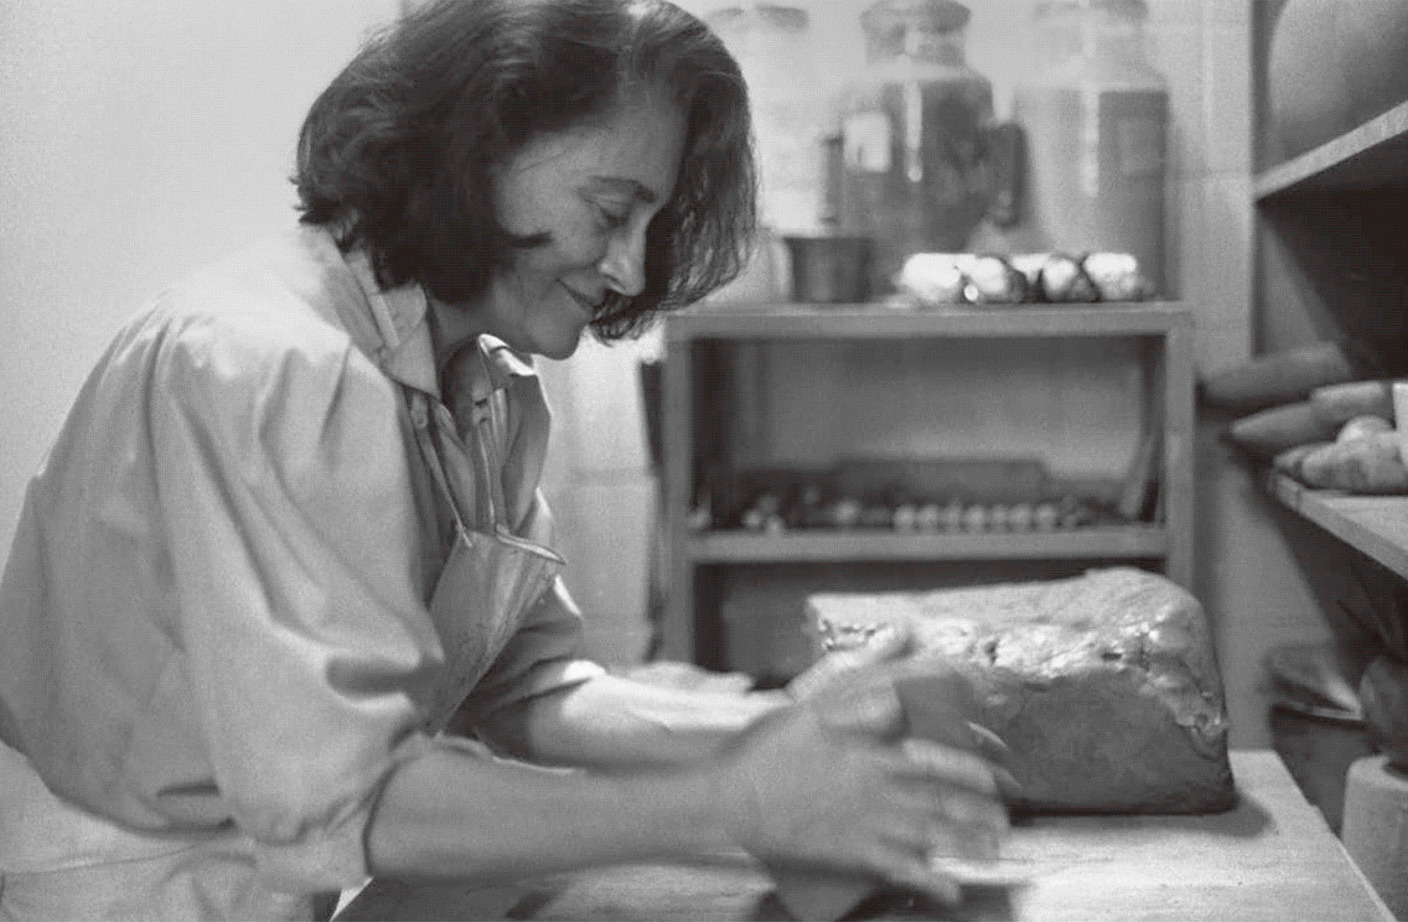
\includegraphics[width=0.8\linewidth]{../../figures/Celeida.jpg}
  \caption{Celeida Tostes em seu ateliê. Fotografia de  Sonia D’Almeida / CPDoc JB, (1987).}
  \label{fig:celeida}
\end{figure}

\section*{O barro como símbolo e mito}
O barro, mais do que simples matéria-prima ou recurso utilitário, ocupa um lugar singular na imaginação humana. Presente desde os mitos de criação como matéria de origem, de transformação e de retorno, ele não é apenas substância moldável, mas também matriz criativa e campo de projeção arquetípica. A experiência simbólica que dele brota exige uma abordagem situada na subjetividade, dimensão essencial para a leitura de obras que o tomam como núcleo, como ocorre em Passagem. Embora resista a análises redutoras, a subjetividade foi explorada por diversas correntes filosóficas e psicológicas que reconheceram no símbolo uma linguagem própria do vivido \parencite{sassFlawGreatDiamond2022}.

Na modernidade, escritores como Proust, Valéry e pintores como Cézanne transformaram a subjetividade em tema da criação, antecipando preocupações que seriam aprofundadas pela fenomenologia e pelo existencialismo. Esse movimento abriu caminho para que o símbolo fosse pensado como presença viva da subjetividade na experiência íntima do sujeito. Convém, aqui, diferenciar o signo e a alegoria do símbolo: este não aponta para além de si, mas participa da própria realidade que manifesta. Goethe sintetizou essa ideia ao afirmar que “os símbolos são aquilo que representam” (apud Sass, 2022, p.25, tradução nossa). Diferentemente do signo ou da alegoria, que remetem a significados fixos, o símbolo se abre ao indeterminado, transmitindo um sentido vivo e múltiplo.

A psicologia analítica acrescenta outra camada a essa discussão. Para Jung, o símbolo nunca esgota seu significado, apontando sempre para algo além de qualquer conceito \parencite[p.60]{jacobiComplexoArquetipoSimbolo2021}. Edinger \citeyear{edingerEgoArchetypeIndividuation1992} explica que ele oferece sentido à vida vivida não como um significado fixo, mas como uma abertura para o desconhecido, situada na própria subjetividade. Embora a teoria da psique de Jung preserve um modelo estrutural e transcendente do inconsciente, sua prática privilegia a escuta simbólica, aproximando-se, nesse ponto, da postura fenomenológica que é reconhecer no símbolo um processo vivo, no qual interior e mundo se encontram na experiência do sujeito.

\begin{quote}
  O símbolo é sempre um produto de natureza extremamente complexa, uma vez que nele intervêm dados de todas as funções psíquicas. […] O símbolo vivo não pode nascer numa mente apática ou pouco desenvolvida, pois tal mente se contentará com os símbolos já existentes oferecidos pela tradição estabelecida. Apenas o anseio apaixonado de uma mente altamente desenvolvida, para a qual o símbolo tradicional já não é a expressão unificada do racional e do irracional, do mais elevado e do mais baixo, pode criar um novo símbolo (Jung, 1967, §825, tradução nossa).
\end{quote}

Podemos considerar o trabalho artístico como um movimento que transcende a elaboração conceitual do símbolo e encontra, na concretização da obra, o espaço onde o gesto criativo une presença material e potência simbólica. Essa perspectiva é amplamente explorada na arteterapia de orientação junguiana, que, no Brasil, teve em Nise da Silveira sua principal pioneira. Ao reconhecer nas imagens produzidas por pacientes psiquiátricos símbolos vivos e não apenas sintomas, sua metodologia abriu caminho para uma prática terapêutica que valoriza a criação artística, a escuta sensível e a importância da materialidade (Silveira, 2015). Hoje difundida em ateliês, escolas e contextos terapêuticos, a arteterapia destaca-se por valorizar não apenas a interpretação de conteúdos inconscientes, mas também a experiência da co-criação entre sujeito e matéria. Como observa Urrutigaray (2023), nessa abordagem o símbolo não é um enigma a ser decifrado, mas uma presença que se manifesta no corpo, na matéria e no tempo da criação.

Gouvêa (2021), ao citar Anaxágoras, “o homem pensa porque tem mãos” (p.68) acrescenta que o fazer manual não é a simples execução de uma ideia, mas pensamento que se dá no entrelaçamento de corpo, matéria e mundo. A mão imprime na matéria o que não pode ser elaborado em palavras; no contexto terapêutico, projeta conteúdos inconscientes em formas sensíveis. Criar com as mãos é, assim, mais do que produzir objetos: é instaurar uma linguagem em que a matéria se torna mediadora entre o subjetivo e o concreto.

Por sua resistência plástica ao tato e por instaurar uma temporalidade própria na interação, o barro ocupa um lugar privilegiado. Modelar não se limita à obtenção de uma forma final: abre uma fenda simbólica em que imagens germinam e se transformam. Nesse gesto, o ato individual de moldar a terra reflete, em escala íntima, narrativas coletivas e ancestrais, fruto da longa relação da humanidade com esse elemento. Essa matéria úmida e escura, tradicionalmente associada ao feminino, ao útero e à Lua, carrega um saber ancestral que convida à coautoria entre sujeito e mundo: “No barro, o homem cria e é criado” (Gouvêa, 2021, p.73).

Não por acaso, mitos de diferentes tradições situam o barro como matéria primordial da criação. No antigo Egito, o deus Khnum era o oleiro divino que moldava os corpos humanos em seu torno, usando o lodo fértil do Nilo. Na tradição judaico-cristã, Adão, cujo nome deriva da palavra hebraica adamah (terra), é formado do pó do solo e recebe o sopro divino como vida. 

A força desses mitos não reside apenas em suas narrativas, mas, segundo a psicologia analítica, em sua capacidade de ativar imagens do inconsciente coletivo — camada profunda da psique que abriga conteúdos transpessoais e arquetípicos (Jung, 2007). Os arquétipos, por sua vez, constituem as formas estruturais desse inconsciente: padrões universais de experiência que não possuem conteúdo fixo, mas se atualizam em mitos, sonhos e símbolos sempre que encontram uma situação existencial correspondente na vida do sujeito. Desse modo, para a psicologia analítica, os mitos operam como narrativas coletivas que dão corpo a essas potências, oferecendo imagens através das quais o indivíduo pode elaborar o que permanece latente em sua psique.

Ainda entre as narrativas que vinculam o barro à criação da humanidade, destaca-se, na cosmologia iorubá, o mito de Nanã, segundo o qual os corpos humanos só puderam ser moldados a partir da lama primordial, pois apenas essa matéria era capaz de acolher a vida. Trazido ao Brasil pela diáspora forçada da escravidão atlântica, esse mito enraizou-se no imaginário afro-brasileiro, tendo o barro como símbolo da ancestralidade, do feminino e da ligação entre origem e morte, entendida como o retorno inevitável do ser humano à terra. Na psicologia analítica, essa dimensão corresponde à Grande Mãe primeva \parencite{zacharias2025}, arquétipo estudado exaustivamente por Erich Neumann, discípulo de Jung, em A Grande Mãe (1955/2015).

Neumann identifica na figura da Grande Mãe a primeira forma estruturante da psique coletiva, uma matriz urobórica a partir da qual se diferenciam tanto o masculino quanto outras manifestações do feminino. A partir dessa genealogia, o autor percorre culturas, objetos rituais, esculturas e pinturas, reconhecendo múltiplas expressões do arquétipo. Sobre essa figura projetam-se aspectos ambivalentes: ora fonte de vida, cuidado e sabedoria; ora força destrutiva, possessiva e cruel. Essa polaridade não constitui um simples contraste, mas uma tensão essencial ao feminino arquetípico. Neumann formula ainda a equação simbólica “mulher = corpo = vaso = mundo”, mostrando como esses elementos funcionam como recipientes equivalentes, espaços de germinação, abrigo e cuidado.

Na criação de Celeida, vemos a reinterpretação poética dessa equação simbólica. O barro, enquanto matéria informe, remete à origem de toda criação; o vaso, ao ganhar forma, torna-se ventre de gestação e imagem do feminino como potência transformadora. É nessa atitude profundamente simbólica de entrar nua neste recipiente, permanecer em seu interior e rompê-lo para renascer que Celeida ressignifica o arquétipo feminino no horizonte da arte de seu tempo.

\section*{Celeida e o Rio dos anos 1970}
Ao trazer a cerâmica para o espaço da performance e da instalação, Celeida articula o cenário das artes de vanguarda do Rio de Janeiro dos anos 1970 à sua trajetória pessoal, marcada por viagens, leituras e pela experimentação constante com o barro. A argila torna-se uma amálgama que media dimensões simbólicas e concretas, ligando a criação da artista ao tecido social de seu tempo.
Seu trabalho dialoga com debates críticos da época, que defendiam uma arte experimental e aberta, em contraposição aos modelos tradicionais e hierárquicos de representação e apreciação. Nesse horizonte, aproximava-se das proposições de Frederico Morais — como nos eventos do Museu de Arte Moderna do Rio, Domingos de Criação (1970), e na mostra Do Corpo à Terra (1971), no Parque Municipal de Belo Horizonte —, bem como das heranças do neoconcretismo e do espírito experimental e híbrido da Tropicália.

Essa atitude vanguardista dos artistas da época contrastava com o contexto brasileiro da ditadura militar. Nos anos 1970, o país vivia a transição entre o auge da repressão política e do crescimento econômico para, já na segunda metade da década, sob o governo do general Ernesto Geisel, mergulhar em crise econômica e iniciar a chamada “distensão”, projeto dos militares que visava a uma abertura lenta e controlada rumo ao governo civil.

Ao mesmo tempo, a chamada segunda onda do feminismo (1960–1980) ampliava a luta das mulheres para além dos direitos civis e políticos, trazendo à tona pautas como a liberdade sexual, o direito ao aborto e a crítica ao patriarcado, sob o lema “o pessoal é político” (Marques; Xavier, 2018). No Brasil, entretanto, essa assimilação foi mais tardia e atravessada pela censura da ditadura e pela circulação restrita de obras teóricas, sendo mediada por autoras como Heloneida Studart, Rose Marie Muraro e Carmen da Silva, cuja coluna na revista Cláudia difundiu ideias feministas adaptadas ao cotidiano. O estigma da feminista como “violenta” ou “destruidora de lares” levou muitas artistas a evitarem vínculos explícitos com o movimento, embora textos de Carmen da Silva tenham influenciado nomes como Anna Maria Maiolino, Wanda Pimentel, Iole de Freitas e Letícia Parente, que problematizaram o corpo, a vida doméstica e os estereótipos de gênero em plena ditadura (Trizoli, 2012).

Foi nesse cenário, marcado pelas diferentes vertentes do feminismo, pela produção artística das mulheres e pelo ambiente repressivo da ditadura, que Celeida retornou ao Rio de Janeiro, em 1975. Convidada a lecionar na recém-inaugurada Escola de Artes Visuais do Parque Lage, encontrou ali um espaço que rapidamente se consolidaria como um dos núcleos mais férteis de resistência cultural e de reinvenção do ensino da arte no Brasil.

\begin{figure}[ht]
  \centering
  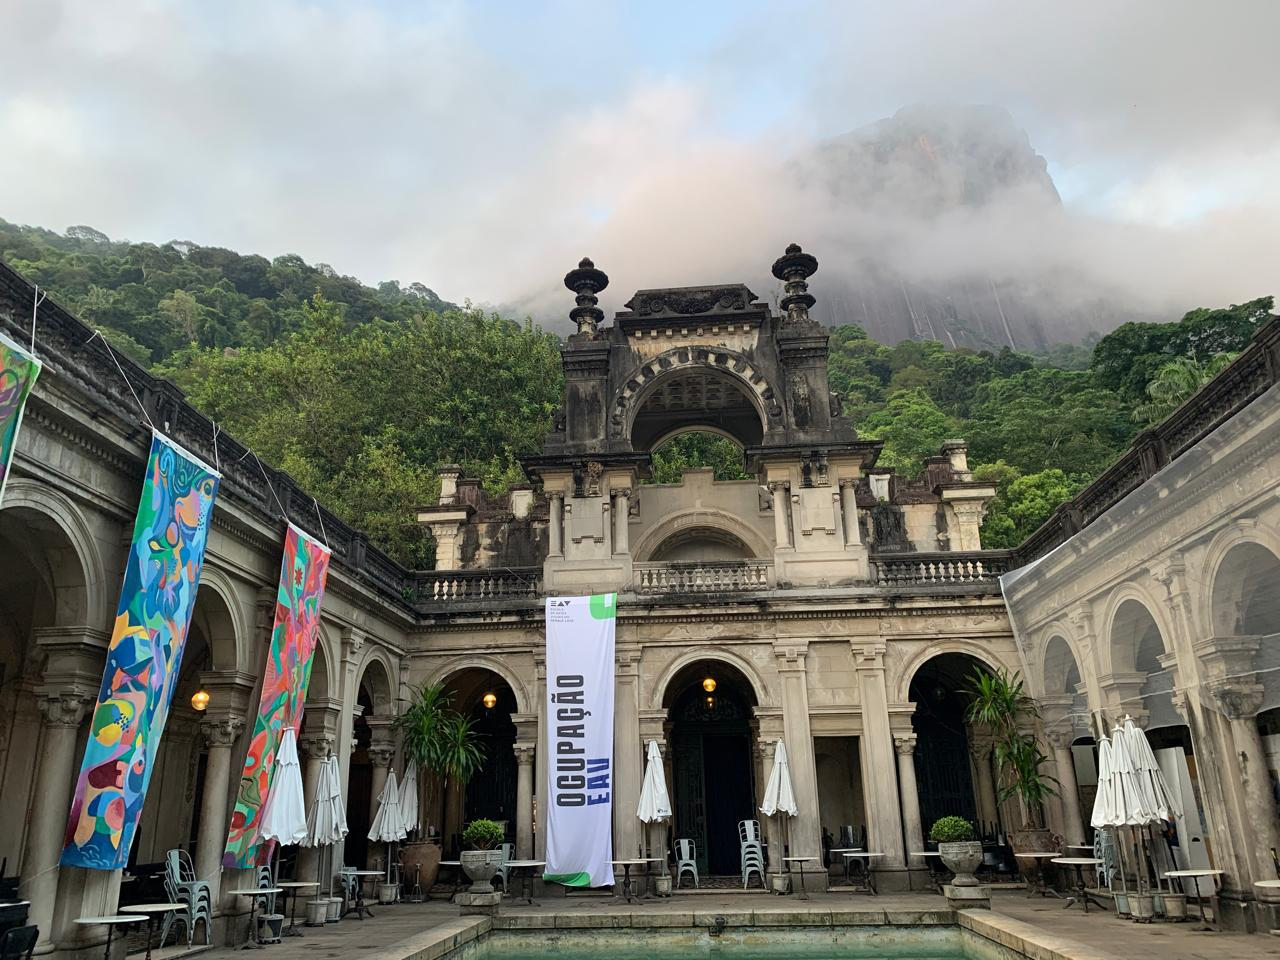
\includegraphics[width=0.8\linewidth]{../../figures/parque_lage.jpg}
  \caption{Escola de Artes Visuais do Parque Lage. Fotografia de Gustavo de Assis (2023).}
  \label{fig:parque-lage}
\end{figure}

Localizada em uma antiga mansão cercada por jardins e pela mata atlântica, a Escola de Artes Visuais do Parque Lage tornou-se um dos principais espaços de liberdade criativa durante a ditadura militar. A transferência da Escola de Belas Artes e de outros cursos da Universidade Federal do Rio de Janeiro para o campus isolado da Ilha do Fundão contribuiu para esse papel: em contraste com esse afastamento, o Parque Lage emergiu como um dos poucos espaços urbanos abertos, articulando em seus programas de ensino uma prática crítica e experimental. Diferentemente do modelo acadêmico tradicional, estruturava-se como um ambiente de ensino horizontal e coletivo, em que professores e alunos compartilhavam oficinas, debates e práticas artísticas interdisciplinares. Sua pedagogia não se restringia ao domínio técnico, mas dialogava com modelos como o Black Mountain College, reinterpretados à luz da realidade brasileira e das experiências de criação artística fora da academia.

Nesse campo didático inovador, lembra Saldanha (2016), a escola dialogava com a experiência pioneira de Nise da Silveira, que, nos anos 1950, criou o Museu de Imagens do Inconsciente, transformando a clínica psiquiátrica em um espaço de produção simbólica e de escuta do inconsciente coletivo. Sua prática ofereceu uma alternativa ao autoritarismo médico e redefiniu o lugar da criação, ao reconhecer nos pacientes internados não apenas sujeitos de tratamento, mas criadores dotados de expressão estética e sensibilidade artística. Além disso, a defesa de uma educação integrada pela arte, proposta por Herbert Read, e a pedagogia libertadora de Paulo Freire, formulada nos anos 1960, fortaleceram o horizonte teórico e prático da escola.

Nesse contexto, a presença de Celeida Tostes foi decisiva para consolidar um espaço sensível às questões da vanguarda. Como recorda Hélio Eichbauer, “a Celeida, com o barro, com a argila, recriou um mundo. Havia uma questão ancestral, o ritual da criação. Isso se tratava muito no começo da escola” (apud Saldanha, 2016, p.277). Sua prática, ao retomar imagens arquetípicas como o “ovo cósmico”, inscrevia-se em diálogo com a psicologia junguiana, articulando o barro às expressões do inconsciente coletivo.

Suas oficinas, baseadas no contato direto com a matéria e na experimentação sensorial, desestabilizavam hierarquias e abriam espaço para processos criativos inesperados. Dessa experiência nasceu o neologismo cunhado pelo colega e pintor Luiz Áquila: celeidar, verbo que sintetizava sua potência pedagógica: mais do que ensinar técnicas, tratava-se de provocar deslocamentos e abrir caminhos de criação coletiva. Sua sala de aula funcionava como um ateliê compartilhado, no qual processo e escuta ocupavam lugar central. Criar obras de arte significava também transformar a si mesmos, inclusive Celeida, enquanto mediadora desse processo. 

O que nascia no Parque Lage como prática coletiva encontraria, pouco depois, um novo campo de ação: a comunidade do Chapéu Mangueira, no Leme, onde ela implantou um núcleo de cerâmica utilitária junto às mulheres da favela. O trabalho refletia o mesmo princípio vivido no Parque Lage: um aprendizado em via de mão dupla. Como recorda Carmen Vargas, uma das assistentes da artista na época, cada participante recriava em barro a sua própria história, de modo que a prática artística não era assistencialista, mas emancipadora. Esse ambiente colaborativo consolidou sua trajetória em obras emblemáticas, reafirmando a dimensão comunitária e não autoral de sua produção (Tejo, 2022). Para Celeida o barro era também uma forma de retorno, uma reconexão com as próprias origens. Nas mãos das mulheres da favela, tornava-se mediador de identidade e de sustento, gesto que se aproximava do pensamento de bell hooks: ensinar sem impor, ouvir as margens como lugares de criação de saberes e de memória (Silva, 2021).

Em Aldeia Furnarius rufus (1981–1990; Figura 3), inspirada no joão-de-barro, Celeida recriou dezenas de casas em espiral e convidou crianças e grupos diversos a construir uma “cidade ideal”, dissolvendo a autoria individual em um processo compartilhado. Já em O Muro (1982), uma imensa construção de tijolos de adobe erguida em mutirão por artistas, alunos e moradores do Chapéu Mangueira, a autoria se dispersou em ação coletiva, e a obra transformou-se em símbolo ambivalente de separação e encontro (Silva, 2006).

\begin{figure}[ht]
  \centering
  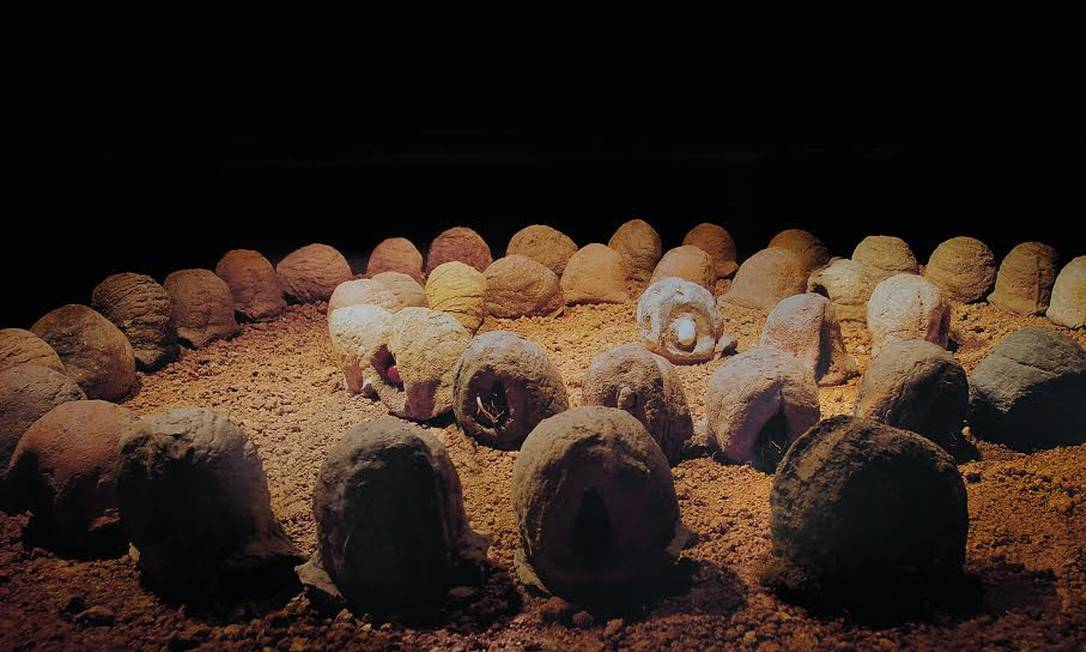
\includegraphics[width=0.8\linewidth]{../../figures/aldeia_furnarius_rufus.jpg}
  \caption{Celeida Tostes, \emph{Aldeia Furnarius rufus}. Instalação exibida na I Bienal do Barro da América, Caracas, 1992. Foto: Divulgação / Acervo Suzete Muzeraqui.}
  \label{fig:furnarius}
\end{figure}

Esse modo de atuar dialogava com o clima político dos anos 1980. Como observa Daniela Name (2014), após décadas de polarização entre capitalismo e socialismo e da repressão da ditadura, a militância se deslocava da praça pública para esferas íntimas e comunitárias. A política passava a ser exercida no cotidiano, nos coletivos artísticos e nas redes de afetos. É nesse contexto que a docência de Celeida se insere, convertendo a sala de aula em ateliê partilhado e projetando esse espaço para a rua e a comunidade, em um movimento de criação coletiva, pensamento crítico e liberdade — atitudes que, em pleno regime autoritário, soavam subversivas.

Essa fusão entre criação e vida, intensificada a partir do final dos anos 1970, reencontra uma linhagem aberta décadas antes pelo neoconcretismo. Desde o final dos anos 1950, artistas como Lygia Clark, Lygia Pape e Hélio Oiticica propuseram uma arte que deixava de ser objeto autônomo para tornar-se experiência sensível. Definida como “não-objeto” por Ferreira Gullar e como “proposição” por Oiticica, esse movimento deslocou o foco do objeto para o corpo e para a participação do público, transformando a figura do artista de “gênio criador” em propositor ou educador (Cayses, 2014). Essa afinidade manifesta-se também na valorização do processo, da experiência fenomenológica e da presença no espaço vivido, em consonância com a filosofia de Merleau-Ponty (Gullar, 1959). Assim como os neoconcretos buscaram romper com o formalismo construtivo para aproximar a arte do mundo vivido, Celeida enfatizou o processo, o corpo e a partilha como núcleos de criação.

Sob esse enfoque, a artista revela afinidades diretas com os experimentos de Lygia Pape e Lygia Clark. Como observa Name (2014), “há uma ligação bastante potente entre Passagem e as experiências Ovo, de Lygia Pape, e A casa é o corpo, de Lygia Clark” (p. 58). Em todos esses casos, o corpo atravessa um espaço simbólico, transformando a estética em acontecimento e colocando em crise a noção de obra de arte como objeto autônomo e mercadoria. Ao deslocar o valor da arte do produto para a experiência compartilhada, essas artistas recusam a lógica capitalista de produção e consumo, substituindo-a por uma economia do gesto, da partilha e do afeto. Nesse sentido, Passagem partilha da mesma subversão presente nas proposições de Clark e Pape: afirmar-se como gesto político e anticapitalista, ao deslocar a arte de sua função produtora de objetos inseridos na lógica mercantil para o campo do acontecimento — espaço de experiências sensíveis, coletivas e femininas.

\section*{A obra \emph{Passagem} (1979)}
Realizada em seu apartamento em Botafogo e registrada pelo fotógrafo Henry Stahl, a ação contou com a ajuda de duas assistentes. Com elas, Celeida ergueu uma grande ânfora pelo método do acordelado, técnica tradicional de modelagem em que a forma é construída pela sobreposição de rolos de barro. Em seguida, cobriu o corpo com argila líquida e se colocou nua dentro da peça, que foi selada. Após permanecer algum tempo em seu interior, rompeu as paredes e deslizou para fora. Em relatos posteriores, Celeida afirmou ter sido transformada pela experiência, inaugurando um período de aprofundamento em sua relação com a argila.

A ampliação do vaso à escala humana simboliza a passagem da arte para a elaboração simbólica, revelando como a performance de Celeida expande o gesto artístico para o domínio do terapêutico. Nessa perspectiva, evidencia-se uma dinâmica próxima à arteterapia de Nise da Silveira, em que a matéria, em contato com o corpo, atua como veículo de elaboração psíquica. No caso de sua paciente Adelina Gomes (1916–1984), Nise reconheceu que foi por meio da modelagem do barro que ela acessou camadas mais profundas do psiquismo, nas quais a identificação com a figura materna a conduziu ao arquétipo da Grande Mãe. As figuras de Adelina apresentam um arcaísmo que remete às deusas-mãe do período paleolítico, mulheres corpulentas e majestosas associadas às diversas Vênus pré-históricas (Lousa; Mikosz, 2022, p.236). Nesse contexto, o barro fazia emergir imagens maternas em meio à fragmentação de uma psique marcada pela esquizofrenia.

O gesto de Celeida se dá em outro registro: é um movimento consciente de mergulho e retorno, no qual o barro se torna veículo de travessia e criação artística. Sua declaração após a performance — “tive contato com alguma coisa que era como um útero […] Eu acho que trepei com o barro” (Ferreira; Silva, 2014, p. 225) — pode ser lida como uma experiência urobórica, em que a consciência se dissolve na indiferenciação primordial e os opostos se confundem no arquétipo da Grande Mãe. O vaso torna-se, assim, não apenas uma cápsula de travessia, mas também um espaço de fusão erótica e extática, atualização corporal de um estado psíquico em que corpo e mundo ainda não se separaram.

Em contraste, o masculino comparece apenas como guardião da imagem. Henri Stahl fotografa, e seu testemunho silencioso apenas entrevê o aspecto misterioso da experiência, acentuando a centralidade feminina da obra. Essa configuração de gêneros, realizada no espaço doméstico, ressignifica o lugar onde, segundo bell hooks, se aprende e naturaliza o sexismo. Para a autora, o capitalismo retira dos homens o controle sobre a esfera pública e os leva a buscar compensação por meio da violência e da dominação na esfera privada, mantendo a família como locus de opressão patriarcal (Silva, 2021). Ao ocupar esse espaço não para repetir a lógica da subjugação, mas para instaurar um rito de criação e travessia, Celeida requalifica simbolicamente o lar como lugar de criação e liberdade.

É nesse entrelaçamento de presenças, afetos e interpretações que o símbolo revela sua vitalidade: não como imagem fixa, mas como forma em processo, que não substitui um conteúdo já dado. Antes, indica o que pode emergir de sua potência. Seu papel é prospectivo: suscitar sentidos, reativar o processo de conhecimento e abrir caminhos para a subjetividade. O mais fecundo não é decidir se o vaso é útero, túmulo, travessia ou registro do feminino, mas reconhecer que pode ser tudo isso ao mesmo tempo — e ainda outra coisa para cada olhar. Os símbolos, como vasos comunicantes, não se encerram em equivalências rígidas; permitem, antes, que os sentidos circulem e se renovem.

\begin{figure}[ht]
  \centering
  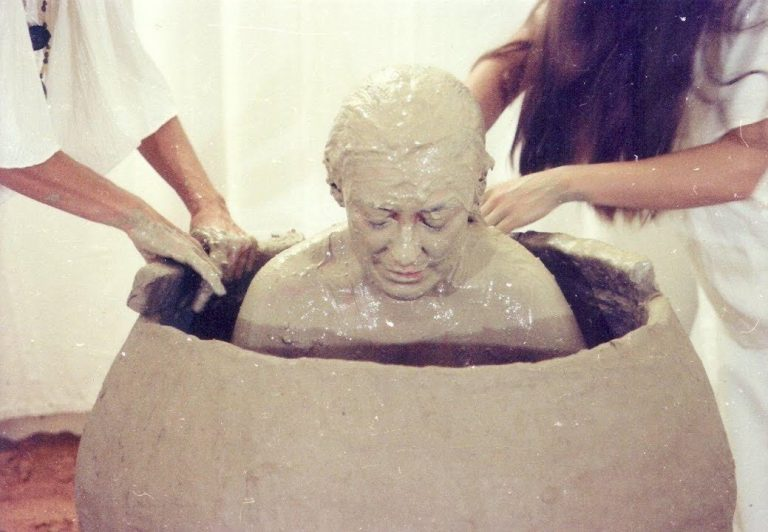
\includegraphics[width=0.8\linewidth]{../../figures/passagem_1.png}
  \caption{Celeida Tostes, Passagem, performance, 1979. Fonte: Extraído de O Relicário de Celeida Tostes (2015, 4min37s).}
  \label{fig:passagem-1}
\end{figure}

Somado a isso, Passagem adquire também uma dimensão política do feminino: em plena ditadura, quando o corpo era alvo de censura e controle, Celeida reivindica a nudez não como motivo erótico, mas como afirmação de um sujeito criador. Ao colocar-se nua dentro de um vaso de barro, confronta o moralismo patriarcal da época e situa o corpo feminino como matriz simbólica e produtiva, em diálogo com as críticas feministas que circulavam no ambiente artístico latino-americano. Se o feminismo, assim como a arte, buscava ampliar seu alcance para incluir questões do cotidiano e da intimidade, Celeida traduz esse movimento para a linguagem do barro, onde o íntimo se torna público e o simbólico se faz coletivo. Sua obra não replica discursos estrangeiros: emerge da realidade brasileira, evocando tanto as urnas funerárias indígenas quanto os rituais afro-brasileiros ligados à terra, e articula barro, corpo feminino e pedagogia em uma poética que reatualiza o feminino arquetípico.

Décadas depois, autores estrangeiros como Suzi Gablik e Michel Maffesoli ofereceram chaves para compreender as tensões entre espiritualidade, coletividade e essencialismos que também atravessam a recepção da obra de mulheres artistas. Em The Reenchantment of Art (1991), Gablik defende uma arte espiritual, comunitária e ecológica, próxima de certas vertentes ecofeministas, embora criticada por reproduzir dualismos como natureza/feminino versus cultura/masculino. Já Maffesoli propõe um “reencantamento do mundo” baseado em identidades plurais e relacionais, enraizadas em mitos, imaginários e formas de sociabilidade afetiva (Trizoli, 2011). Essa dimensão também se faz presente no trabalho de Celeida: embora haja uma identificação do vaso com o útero, sua intervenção evoca igualmente a imagem de um corpo coletivo da terra, lugar de comunhão com a origem, com o feminino arquetípico e com a memória primeira dos seres vivos. A artista nos lembra de uma força subterrânea que pulsa em cada nascimento, nos gestos de cuidado e no retorno à terra, como nos mitos de Nanã.

Para compreender o aspecto processual da obra, é preciso atentar também para a técnica ancestral do acordelado utilizada na moldagem do vaso. Transmitida por mulheres indígenas \parencite{dutraPalcoAoBarro2022}, essa prática, repetitiva, lenta e fisicamente exigente, envolve todo o corpo e conduz a um estado de imersão sensível, em que o sentido da obra não se fixa em um projeto prévio, mas emerge da experiência vivida. Essa valorização do processo também se evidencia em sua prática pedagógica. Como lembra Ricardo Ventura, ex-aluno da Oficina da EAV das Artes do Fogo, parte do método de Celeida consistia justamente em estimular o desapego à ideia de “obra pronta”. Ele recorda que, ao vê-lo contemplar satisfeito uma peça recém-concluída, Celeida a derrubou no chão, reduzindo-a a cacos. O gesto, que num primeiro momento provocou raiva, revelou depois sua lição: o essencial não era o objeto acabado, mas o processo, o caminho, a transformação que o fazer instaurava (Name, 2014, p.56).

\begin{figure}[ht]
  \centering
  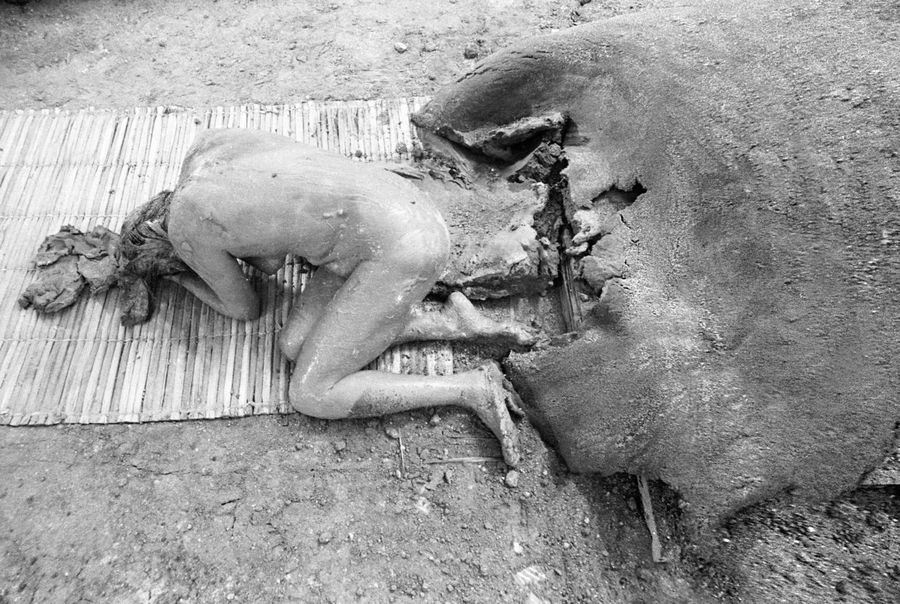
\includegraphics[width=0.8\linewidth]{../../figures/passagem_2.jpg}
  \caption{Celeida Tostes, Passagem, 1979. Fotografia de Henri Stahl.}
  \label{fig:passagem-2}
\end{figure}

É nesse ponto que a performance pode ser lida à luz da noção de quasi-corpus, desenvolvida por Lygia Clark no âmbito do neoconcretismo. Para Clark, o termo designa uma categoria liminar entre obra e corpo: o objeto artístico deixa de ser autônomo e passa a existir apenas no acontecimento da experiência. Nem corpo biológico nem escultura autossuficiente, trata-se de uma entidade híbrida, ativada pela interação. Nessa atitude, Celeida radicaliza o princípio: o vaso de barro não é um simples recipiente, mas um corpo-outro que envolve, contém e é rompido pelo corpo da artista. A fusão entre corpo e matéria, mediada pela técnica do acordelado, cria um espaço fenomenológico em que sujeito e objeto se confundem.

Finalmente, vale recorrer às próprias palavras de Celeida, escritas após a ação, para perceber como sua criação não se apresentava como objeto acabado, mas como experiência de dissolução e recomposição de limites — inclusive formais:

\begin{quote}
  Despojei-me\\
  Cobri meu corpo de barro e fui.\\
  Entrei no bojo do escuro, ventre da terra.\\
  O tempo perdeu o sentido de tempo.\\
  Cheguei ao amorfo.\\
  Posso ter sido mineral, animal, vegetal.\\
  Não sei o que fui.\\
  Não sei onde estava. Espaço.\\
  A história não existia mais.\\
  Sons ressoavam. Saíam de mim.\\
  Dor.\\
  Não sei por onde andei.\\
  O escuro, os sons, a dor, se confundiam.\\
  Transmutação.\\
  O espaço encolheu.\\
  Saí. Voltei.\\
  (Celeida Tostes apud \citeauthor{dutraPalcoAoBarro2022}, 2022, p.15)
\end{quote}

Esse testemunho acentua o caráter processual da obra, não pela fixação de uma forma, mas pelo mergulho no amorfo e naquilo que se transforma incessantemente. É a partir dessa dimensão que podemos compreender Passagem também à luz do termo informe, criado por Georges Bataille (1897–1962). Lançado nos anos 1920 como verbete do Dictionnaire critique, o informe não designa um conceito fixo, mas um gesto de “trazer as coisas para baixo”, desmontando categorias elevadas e recusando significados estáveis. Revisitado por Krauss e Bois (1997) na exposição L’informe: mode d’emploi, o termo foi mobilizado para expor as fissuras do próprio modernismo, mostrando como a arte já continha forças capazes de desestabilizar a oposição entre formalismo e iconologia.

No campo artístico, informe não é simples ausência de forma, mas aquilo que perturba as hierarquias entre forma e matéria, liberando resíduos, manchas, restos e processos inacabados como operadores estéticos. Em oposição à promessa modernista de uma essência autônoma da arte, propõe uma abertura crítica em que a matéria resiste a qualquer desenho prévio. Nesse sentido, Passagem pode ser lida como profundamente informe: o barro, material comum e alheio ao circuito nobre das belas-artes, torna-se operador de desestabilização, recusando a idealização formal e deslocando a criação para o terreno da experiência.

Por fim, essa performance permite reconhecer uma zona de convergência e tensão entre a psicologia analítica e o pensamento do informe. Em Jung, o fluxo encontra configuração simbólica: os arquétipos são “leitos de rios que canalizam o fluxo da vida psíquica segundo os seus próprios padrões. São as formas pré-existentes que dão configuração à massa psíquica amorfa” (1981, §99, tradução nossa). Já em Bataille, o fluxo corrompe e desordena qualquer estrutura: o informe nomeia a recusa de toda forma estável e abre espaço para o transbordamento da matéria e para o gesto que dissolve hierarquias. Passagem habita justamente essa fricção do fluxo, tornando-se imagem viva tanto a psique quanto a matéria, e fazendo da criação um processo em constante transformação.

\section*{Conclusão}
A ação de Celeida condensa as tensões políticas e as potências poéticas que atravessavam o Brasil dos anos 1970 — a ditadura militar, as primeiras articulações feministas e o diálogo com a herança neoconcreta. Enquanto o neoconcretismo buscava dissolver as fronteiras entre arte e vida pela via da percepção e da experiência fenomenológica, Celeida desloca esse impulso para o campo simbólico e espiritual, fazendo de Passagem um rito de transformação que conjuga corpo, matéria e memória.

Na década de 1970, a artista introduz o barro no circuito artístico brasileiro como mediador de identidades e coletividades — gesto que se expande na década seguinte em obras como Aldeia Furnarius rufus e O Muro. Trata-se de um horizonte comum que valoriza o processo com o barro, no qual experiências sociais silenciadas são convocadas à participação criativa. Em Passagem, a artista associa seu trabalho tanto à cerâmica indígena quanto ao fazer manual de mulheres em contextos periféricos, inscrevendo o barro — matéria humilde e cotidiana — no cenário da arte contemporânea. Ao fazê-lo, legitima saberes e vivências marginalizadas e amplia o campo simbólico e político da arte.

A partir desse gesto, sua obra também suscita uma reflexão sobre as experiências de gênero dos participantes e do público, que, ao dialogarem com essa realidade, revelam sua distribuição assimétrica e mobilizam afetos e intensidades distintas conforme as posições interseccionais de cada sujeito no mundo.

Além disso, em Passagem, ao adentrar um vaso de argila e deixar-se envolver pela matéria, a artista assume uma postura de entrega, próxima aos mitos de katábasis como uma descida ritual ao interior da terra e do inconsciente. A leitura de Neumann (1994) esclarece o alcance dessa entrega: ser filho ou filha da terra implica reconhecer nossa condição frágil e compartilhada. A performance encarna essa atitude ao abdicar do controle formal, deixar-se imprimir pela argila e aceitar o peso da matéria sobre o corpo e sobre nossas histórias.

A originalidade dessa obra está em reconhecer que, sem abdicar de universais mínimos, como a precariedade da vida, a subjetividade e a necessidade de expressão simbólica, ela incorpora, com bell hooks, a compreensão de que o “comum” se manifesta de modos situados e interseccionais, moldados pelas vivências da artista nos diversos contextos do Brasil dos anos 1970. As mediações de gênero, classe, raça e território tornam-se, assim, visíveis, recolocando a precariedade não apenas como condição formal, mas como força subjacente ao próprio processo de criação e produção de sentido. A experiência estética, portanto, reabre-se como encontro entre sujeitos, corpo e mundo, em que a obra explicita posições e relações sem, contudo, encerrá-las, iluminando outras formas de existir e narrar.

O simbólico aqui, longe de marcar limites fixos, reforça essa matriz relacional: condensa gesto, matéria e contexto sem apagar as interseccionalidades mas antes, convocando-as como parte constitutiva da experiência humana. É na abertura do subjetivo que, ao mesmo tempo, nos unem e nos situam, que os símbolos se tornam férteis e se renovam. Como escreve Rilke (1925/1972), somos “abelhas do invisível” quando transmutamos o efêmero da experiência pessoal em matéria sensível, fazendo do vivido relacional uma forma que permanece e continua a gerar sentido. O gesto com o barro, nesse horizonte, não é apenas ação exterior, mas condição para a elaboração e a ampliação de sentido. É por meio da linguagem poética que a terra se faz presença íntima, abrindo as leituras do mundo a novas possibilidades, como no vaso da artista, em cuja metáfora ecoa Rilke:

\begin{citacao}
  A terra não tem outra saída senão tornar-se invisível: \emph{em} nós, que com uma parte de nossa natureza participamos do invisível, temos (ao menos) parte nele, e podemos aumentar nossas reservas do invisível durante nossa estada aqui — somente \emph{em} nós pode consumar-se essa íntima e duradoura conversão do visível em um invisível que já não depende de ser visto e tocado, assim como nosso próprio destino cresce continuamente, ao mesmo tempo MAIS PRESENTE E INVISÍVEL em nós. \parencite[p.445]{rilkeLetterWitoldHulewicz1972}tradução nossa, grifos do original
\end{citacao}

A importância desta obra, enfim, não se limita ao gesto que a originou. Ela nos convida a repensar a crítica de arte como escuta simbólica — não reduzir a criação ao seu conteúdo imediato, mas reconhecê-la como processo vivo e relacional, capaz de reativar sentidos latentes e instaurar novas conexões. Assim, a crítica deixa de ser apenas interpretação ou juízo para tornar-se também espaço de abertura, um lugar onde a arte continua a falar e a suscitar respostas, mesmo quando o gesto já se tornou invisível.
 %inclui o arquivo com o conteúdo do artigo
\printbibliography[heading=bibintoc,title={Referências}]

\end{document}
